\documentclass[11pt,a4paper]{article}
\usepackage[margin=20mm,headheight=14pt]{geometry}
\usepackage[T1]{fontenc}
\usepackage{lmodern}
\usepackage{microtype}
\usepackage{xcolor}
\usepackage{booktabs,tabularx,array,longtable}
\usepackage{amsmath}
\usepackage{enumitem}
\usepackage{titlesec}
\usepackage[most]{tcolorbox}
\usepackage{tikz}
\usetikzlibrary{arrows.meta,angles,quotes,positioning,calc,decorations.pathmorphing}
\usepackage[hidelinks]{hyperref}
\usepackage{fancyhdr}
\setlength{\parindent}{0pt}
\setlength{\parskip}{4pt}
\linespread{1.035}
\setlist[itemize]{leftmargin=5mm,itemsep=2pt,topsep=2pt}
\setlist[enumerate]{leftmargin=6mm,itemsep=3pt,topsep=2pt}
\titlespacing*{\section}{0pt}{10pt}{4pt}
\titlespacing*{\subsection}{0pt}{7pt}{3pt}
\titleformat*{\section}{\large\bfseries}
\titleformat*{\subsection}{\normalsize\bfseries}
\definecolor{ink}{HTML}{1D1D1F}
\definecolor{muted}{HTML}{6E6E73}
\definecolor{blue}{HTML}{0071E3}
\definecolor{orange}{HTML}{C65D00}
\definecolor{soft}{HTML}{F5F5F7}
\definecolor{line}{HTML}{D2D2D7}
\definecolor{mist}{HTML}{FFF4E8}
\color{ink}
\newtcolorbox{keybox}[1]{enhanced,breakable,colback=soft,colframe=line,boxrule=.5pt,arc=2mm,title={#1},fonttitle=\bfseries,coltitle=ink,left=3mm,right=3mm,top=2mm,bottom=2mm}
\newtcolorbox{mistakebox}[1][Common mistake]{enhanced,breakable,colback=mist,colframe=orange!55,boxrule=.55pt,arc=2mm,title={#1},fonttitle=\bfseries,coltitle=ink,left=3mm,right=3mm,top=2mm,bottom=2mm}
\newcommand{\band}[1]{\fcolorbox{line}{soft}{\strut\;#1\;}}
\newcolumntype{Y}{>{\raggedright\arraybackslash}X}
\pagestyle{fancy}
\fancyhf{}
\lhead{Electromagnetic Spectrum, Reflection \& Wavefronts}
\rhead{Phuc Nguyen}
\cfoot{\thepage}
\renewcommand{\headrulewidth}{.35pt}
\begin{document}
\begin{center}
{\LARGE\bfseries GCSE Physics --- Electromagnetic Spectrum, Reflection \& Wavefronts}\par
\vspace{2mm}
{\color{muted}Student: Phuc Nguyen \quad Tutor: Alex Kealy \quad Date: 2026-07-16}\par
{\small\color{muted}Source: Loom recording (full video analysis) + transcript}
\end{center}
\small

\section*{1. Electromagnetic spectrum: one family, one fixed order}
Alex described the electromagnetic spectrum as the categories of light: all the light being discussed fits somewhere in this spectrum. The categories are not separate lists to learn for different questions. There is one fixed sequence, and a question merely asks you to travel through that sequence in one direction or the other.

From \textbf{lowest frequency / longest wavelength} to \textbf{highest frequency / shortest wavelength}, the order is
\begin{center}
\band{Radio} $\rightarrow$ \band{Microwave} $\rightarrow$ \band{Infrared} $\rightarrow$ \band{Visible} $\rightarrow$ \band{Ultraviolet} $\rightarrow$ \band{X-ray} $\rightarrow$ \band{Gamma}.
\end{center}
The compact board notation was \textbf{R, M, IR, V, UV, X, $\gamma$}. The essential link is that frequency and wavelength run in opposite directions. Moving from radio towards gamma means frequency is increasing while wavelength is decreasing. Moving from gamma towards radio means frequency is decreasing while wavelength is increasing. This is why ``ascending frequency'' and ``descending wavelength'' produce exactly the same radio-to-gamma answer.

\begin{center}
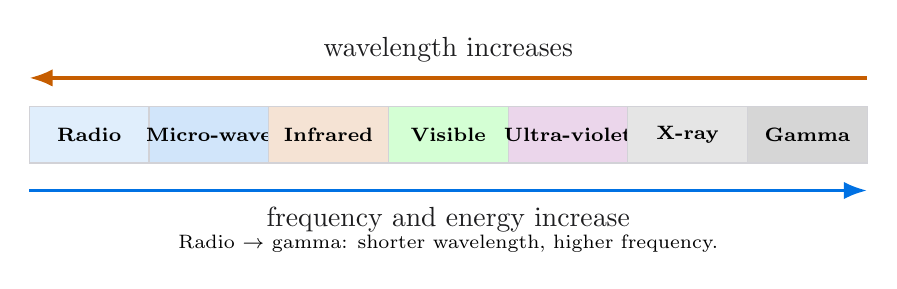
\begin{tikzpicture}[x=1.52cm,y=1cm,>=Latex]
\foreach \x/\lab/\fillc in {0/Radio/blue!12,1/Micro-/blue!18,2/Infrared/orange!17,3/Visible/green!17,4/Ultra-/violet!16,5/X-ray/gray!20,6/Gamma/gray!32}{
  \draw[fill=\fillc,draw=line] (\x,0) rectangle ++(1,.72);
  \node[align=center,font=\scriptsize\bfseries] at (\x+.5,.36){\lab\ifnum\x=1 wave\fi\ifnum\x=4 violet\fi};}
\draw[very thick,blue,-Latex] (0,-.35)--(7,-.35) node[midway,below=2pt,text=ink]{frequency and energy increase};
\draw[very thick,orange,-Latex] (7,1.08)--(0,1.08) node[midway,above=2pt,text=ink]{wavelength increases};
\node[font=\scriptsize,align=center] at (3.5,-1.02){Radio $\rightarrow$ gamma: shorter wavelength, higher frequency.};
\end{tikzpicture}
\end{center}

\subsection*{Frequency, energy and danger}
At the beginning of the recording Alex was finishing the high-frequency end of the board. He explained the threshold in words: by the time we reach ultraviolet, the waves have sufficiently high frequency and sufficiently high energy to remove electrons from atoms. Removing electrons is \textbf{ionisation}. This is the reason the lesson grouped ultraviolet, X-rays and gamma rays as potentially dangerous rather than merely asking for a memorised warning.

The chain of reasoning is:
\begin{center}
\textbf{higher frequency} $\longrightarrow$ \textbf{higher energy} $\longrightarrow$ \textbf{can ionise atoms} $\longrightarrow$ \textbf{cell mutation} $\longrightarrow$ \textbf{possible cancer}.
\end{center}
Visible light is lower in frequency than ultraviolet. In Alex's explanation, visible light has not yet reached the high-frequency, high-energy region that can remove electrons; ultraviolet marks the point at which the ionising danger begins in the ordering used in the lesson. The important exam skill is to give the causal explanation, not to write only ``it is dangerous''.

\subsection*{The completed board rows shown in this lesson}
The video began while the class was continuing an existing spectrum table. The two rows completed and visible in this recording were X-rays and gamma rays, reproduced below with the board wording.

\renewcommand{\arraystretch}{1.28}
\begin{tabularx}{\linewidth}{>{\bfseries}p{.14\linewidth}YY}
\toprule
Band & Uses (board wording) & Danger (board wording)\\
\midrule
X-rays & See bones; industrial imaging & Ionises atoms in cells; mutation -- cancer\\
Gamma rays & Treat cancer; sterilize equipment -- kills bacteria & Ionises atoms in cells; mutation -- cancer\\
\bottomrule
\end{tabularx}

Alex connected each terse entry to a real situation. X-rays can image bones, but the same penetrating imaging idea can be used in industry: machinery can be X-rayed to inspect it. Gamma rays can be used to treat cancer. They can also be shone on surgical tools before an operation to kill bacteria and sterilise the equipment. There is no contradiction between these uses and the danger column. The ability to damage or kill cells can be directed deliberately at cancer cells or bacteria, but exposure can also mutate healthy cells. The desired use and the hazard arise from the same ionising action.

\begin{mistakebox}
Do not say that gamma rays are ``safe because they treat cancer.'' The lesson's table puts \emph{treat cancer} in the use column and \emph{ionises atoms in cells; mutation--cancer} in the danger column. A controlled use does not remove the hazard. Also avoid claiming that X-rays are used only for bones: Alex explicitly added industrial imaging.
\end{mistakebox}

\section*{2. Retrieval drills: how to produce the order under pressure}
Alex did not leave the spectrum as a passive list. He hid the answer and asked for three different orderings. These drills reveal a reliable method: first decide what quantity is changing, then decide which end to start at, and finally check that all seven abbreviations appear exactly once.

\subsection*{Drill 1: ascending frequency}
The question was: \emph{List the categories in the electromagnetic spectrum in order of ascending frequency.}

Phuc began with radio and microwave, but then jumped to X-ray and gamma. Alex did not supply the entire answer; he pointed out that something had been missed in the middle. Phuc recovered the missing region: infrared, visible and ultraviolet. The corrected full answer was
\[
\boxed{\mathrm{R,\ M,\ IR,\ V,\ UV,\ X,\ \gamma}}.
\]
A good walkthrough is: underline \emph{ascending frequency}, start at radio, write R--M--IR--V--UV--X--$\gamma$, then count seven. The count would have caught the actual jump.

\subsection*{Drill 2: descending frequency}
For descending frequency, start at the high-frequency end and reverse the sequence:
\[
\boxed{\mathrm{\gamma,\ X,\ UV,\ V,\ IR,\ M,\ R}}.
\]
Phuc correctly moved gamma through infrared. Near the low-frequency end he almost moved directly to radio; Alex prompted that one category sat between, and Phuc supplied microwaves.

\subsection*{Drill 3: descending wavelength}
The phrase now changed from frequency to wavelength. Phuc first offered microwave, then corrected to radio after Alex's prompt. He then completed microwave, infrared, visible, ultraviolet, X-ray and gamma. The final answer is again
\[
\boxed{\mathrm{R,\ M,\ IR,\ V,\ UV,\ X,\ \gamma}}.
\]
Radio has the longest wavelength, so descending wavelength begins there. Shorter wavelength takes us towards gamma. Alex celebrated the corrected sequence because Phuc had switched quantities correctly.

\begin{keybox}{Alex's memory strategy}
Alex recommended inventing your own story that uses the spectrum bands. He emphasised that a weird or shocking story is more memorable, and that a story made by the learner is better than simply borrowing someone else's. Phuc suggested flashcards; these can test recall, but the story is a separate device for securing the order. Whatever mnemonic you choose, use R--M--IR--V--UV--X--$\gamma$ as the final accuracy check.
\end{keybox}

\begin{mistakebox}
The actual lesson errors were omissions, not a total misunderstanding: Phuc jumped over IR--V--UV in the first drill, nearly omitted microwave in the reverse drill, and initially began descending wavelength at microwave rather than radio. The cure is not faster recitation. Write all seven abbreviations and explicitly translate the direction words before answering.
\end{mistakebox}

\section*{3. Why humans see the visible region: Alex's extension story}
Alex briefly crossed into biology to ask why humans detect visible light but not infrared, ultraviolet or X-rays. Phuc said eye cells detect visible light and convert it into electrical signals for the brain. Alex then added an evolutionary explanation using a graph of absorption by water.

Life began in water, and eyes developed gradually as animals evolved there. On the graph Alex showed, the visible region was the part least absorbed by water; other frequencies tended to be absorbed more. Therefore visible light was the light most available underwater, and evolution developed vision around that available region. This was presented as an explanatory aside, not as a new calculation or a full biology topic. The useful lesson connection is that ``visible'' is not physically separate from the rest of the electromagnetic spectrum: it is the band our eyes evolved to sense.

\begin{mistakebox}
Do not turn Alex's aside into the unsupported claim that humans see visible light simply because it is the only ``safe'' radiation. Phuc suggested safety, but Alex's taught explanation used evolutionary development in water and the relative availability of visible light because it is least absorbed there.
\end{mistakebox}

\section*{4. Rays and wavefronts: two drawings of the same travelling wave}
Before reflection, Alex asked for the difference between rays and wavefronts. He stressed that these are not two different kinds of wave. They are two representations of the same wave behaviour.

A \textbf{wavefront} is a line joining points at the same stage, or phase, of the wave cycle. Looking sideways at repeated ocean waves, one might join every peak. One could instead choose every trough or every equilibrium crossing; the choice is valid provided the same part of each cycle is joined. Looking down on waves spreading from a point, the wavefronts appear as concentric circles.

A \textbf{ray} is an arrow showing the direction in which the wave and its energy travel. Alex's analogy was the \textbf{surfer on the wave}: imagine following the direction in which the surfer is carried. A ray must have an arrowhead because direction is the information it is meant to communicate. Rays are always perpendicular to wavefronts, meeting them at $90^\circ$.

\begin{center}
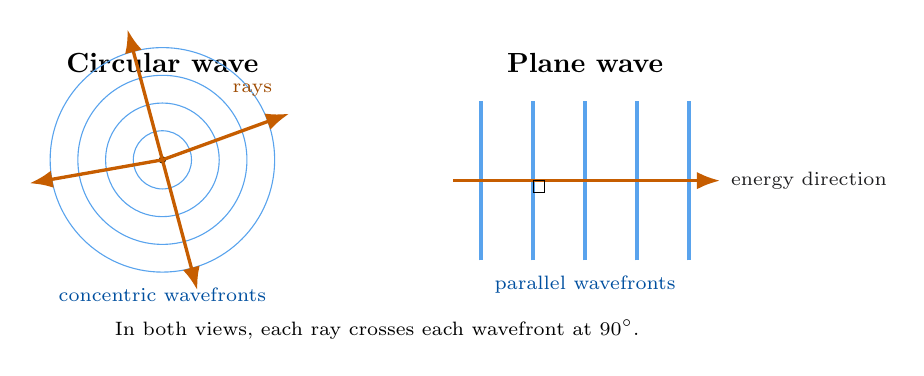
\begin{tikzpicture}[>=Latex,scale=.88]
% circular
\node[font=\bfseries] at (-3.1,2.3){Circular wave};
\fill (-3.1,.9) circle (1.5pt);
\foreach \r in {.42,.82,1.22,1.62}{\draw[blue!65] (-3.1,.9) circle (\r);}
\foreach \a in {20,105,190,285}{\draw[orange,very thick,-Latex] (-3.1,.9)--++(\a:1.95);}
\node[blue!70!black,align=center,font=\scriptsize] at (-3.1,-1.05){concentric wavefronts};
\node[orange!80!black,font=\scriptsize] at (-1.8,1.9){rays};
% plane
\node[font=\bfseries] at (3.0,2.3){Plane wave};
\foreach \x in {1.5,2.25,3,3.75,4.5}{\draw[blue!65,very thick] (\x,-.55)--(\x,1.75);}
\draw[orange,very thick,-Latex] (1.1,.6)--(4.95,.6) node[right,text=ink,font=\scriptsize]{energy direction};
\draw (2.25,.43) rectangle ++(.17,.17);
\node[blue!70!black,font=\scriptsize] at (3,-.9){parallel wavefronts};
\node[font=\scriptsize,align=center] at (0,-1.55){In both views, each ray crosses each wavefront at $90^\circ$.};
\end{tikzpicture}
\end{center}

To draw a plane wave moving right, either draw parallel vertical wavefronts and indicate their movement to the right, or draw a horizontal ray with an arrow to the right. To draw waves spreading from a point, use concentric wavefronts and radial rays. Alex repeatedly recoloured and pointed out both features because each of the lesson diagrams contained both rays and wavefronts.

\begin{mistakebox}
Do not identify an entire picture as ``the ray picture'' or ``the wavefront picture'' without checking its markings: both of Alex's pictures contained both representations. A line without an arrow does not communicate ray direction, and rays drawn parallel to wavefronts are geometrically wrong; they must cross at $90^\circ$.
\end{mistakebox}

\section*{5. Light and materials: luminous, transparent, translucent and opaque}
A \textbf{luminous} object emits or gives off its own light. Alex's examples were the Sun, a light bulb, a candle and fire. This definition separates a source of light from an object that is merely visible. Most objects we see are not producing their own light; light from a luminous source reaches them and is then reflected towards our eyes.

A \textbf{transparent} material transmits light: light goes through it. Alex noted that a little light may also be reflected, which helps us detect that the transparent surface is present, but transmission is the defining behaviour. An \textbf{opaque} material is the opposite: it does not let light pass through. It reflects most of the incident light and absorbs some.

Alex used his pink T-shirt to connect reflection and colour. The opaque shirt absorbs the other colours and reflects pink light towards the observer, so it appears pink. He explicitly kept colour brief, so this guide does not extend that comment into a separate colour theory topic.

Later, Alex briefly mentioned \textbf{translucent} because it can occur in the same vocabulary set. A translucent material is between transparent and opaque: it lets some light through. His example was the cloudy-looking glass of a bathroom window. This was a short extension, not a major assessed section of the lesson.

\begin{tabularx}{\linewidth}{>{\bfseries}p{.18\linewidth}Y Y}
\toprule
Term & What light does & Lesson example or consequence\\
\midrule
Luminous & The object emits its own light. & Sun, light bulb, candle, fire.\\
Transparent & Light is transmitted through; a little may reflect. & We can still detect the surface partly because some light reflects.\\
Translucent & Some light passes through. & Cloudy bathroom-window glass; mentioned briefly.\\
Opaque & Light does not pass through; most reflects and some is absorbed. & A pink shirt reflects pink light and absorbs other colours.\\
\bottomrule
\end{tabularx}

\begin{mistakebox}
Visible does not mean luminous. A pink shirt is visible because it reflects light, not because it emits pink light. Also, transparent does not mean that absolutely no light reflects; Alex explicitly pointed out that a little may be reflected.
\end{mistakebox}

\section*{6. The law of reflection: measure from the ``always'' line}
Alex described physics ``laws'' as observed patterns rather than rules someone ordered nature to obey. For a flat, or \textbf{plane}, mirror, this pattern is the law of reflection.

The incoming ray is the \textbf{incident ray}; Alex linked this to ``in''. The ray leaving the surface is the \textbf{reflected ray}, the ray going ``out''. At the exact point where the incident ray touches the mirror, draw the \textbf{normal}: an imaginary line at $90^\circ$ to the surface. The angle between the incident ray and the normal is the angle of incidence, $i$. The angle between the normal and the reflected ray is the angle of reflection, $r$.
\[
\boxed{\text{angle of incidence}=\text{angle of reflection}\qquad i=r}
\]

\begin{center}
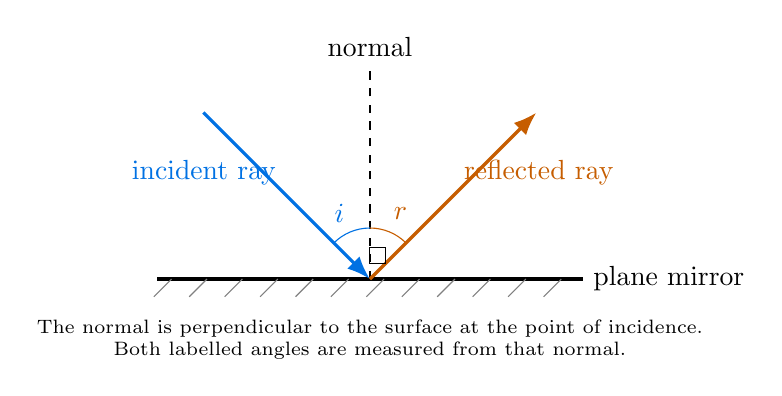
\begin{tikzpicture}[>=Latex,scale=.9]
\draw[very thick] (-3,0)--(3,0) node[right]{plane mirror};
\foreach \x in {-2.8,-2.3,...,2.7}\draw[gray] (\x,0)--++(-.25,-.25);
\draw[dashed,thick] (0,0)--(0,3) node[above]{normal};
\draw[very thick,blue,-Latex] (-2.35,2.35)--(0,0) node[midway,above left]{incident ray};
\draw[very thick,orange,-Latex] (0,0)--(2.35,2.35) node[midway,above right]{reflected ray};
\draw[blue] (0,.72) arc[start angle=90,end angle=135,radius=.72];
\draw[orange] (0,.72) arc[start angle=90,end angle=45,radius=.72];
\node[blue] at (-.43,.92){$i$};
\node[orange] at (.43,.92){$r$};
\draw (0,.22) rectangle ++(.22,.22);
\node[font=\scriptsize,align=center] at (0,-.85){The normal is perpendicular to the surface at the point of incidence.\\Both labelled angles are measured from that normal.};
\end{tikzpicture}
\end{center}

Alex joked that the normal has the wrong name and should be called the \textbf{``always''}: angles are always measured from it. This matters especially when a surface is curved or rough. The normal must be constructed at the exact point where that particular ray hits, perpendicular to the local surface there. The mirror may change shape, but the law can still be applied ray by ray using the correct local normal.

\begin{keybox}{Step-by-step reflection construction}
\begin{enumerate}
\item Mark the precise point where the incident ray meets the surface.
\item Draw the normal through that point, at $90^\circ$ to the surface.
\item Measure the angle between the incident ray and the normal; call it $i$.
\item On the other side of the normal, construct the reflected ray so that $r=i$.
\item Add arrowheads: incident points towards the mirror; reflected points away.
\end{enumerate}
\end{keybox}

\begin{mistakebox}
The most important warning in this section is Alex's ``always'' rule. Measuring from the mirror surface gives the complementary angle and is a common exam error. The normal is not an arbitrary vertical line either: it is perpendicular to the surface at the actual point of incidence.
\end{mistakebox}

\section*{7. Specular and diffuse reflection: the law still works locally}
\textbf{Specular reflection} occurs at a smooth surface. In Alex's diagram, parallel incident rays struck a perfectly flat mirror. Because the surface orientation was the same at every impact point, the normals were parallel. Each ray obeyed $i=r$, so the reflected rays remained parallel and travelled in one ordered direction. This ordered pattern is what allows a clear image in a mirror.

\textbf{Diffuse reflection} occurs at a rough surface. Parallel rays arrive together, but each strikes a small part of the surface tilted differently. Each local normal therefore points in a different direction. Applying $i=r$ around those different normals sends the reflected rays in many directions: the light is scattered. Alex connected this to ordinary objects, most of whose surfaces are rough rather than perfect mirrors. We see light spread in many directions instead of a clear mirrored image.

\begin{center}
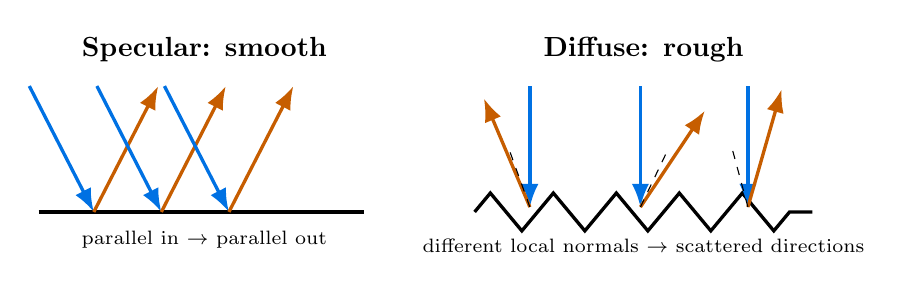
\begin{tikzpicture}[>=Latex,scale=.78]
% specular
\node[font=\bfseries] at (-3.7,2.65){Specular: smooth};
\draw[very thick] (-6.4,0)--(-1.1,0);
\foreach \x in {-5.5,-4.4,-3.3}{
 \draw[blue,very thick,-Latex] (\x-1.05,2.05)--(\x,0);
 \draw[orange,very thick,-Latex] (\x,0)--(\x+1.05,2.05);}
\node[font=\scriptsize] at (-3.7,-.45){parallel in $\rightarrow$ parallel out};
% diffuse
\node[font=\bfseries] at (3.45,2.65){Diffuse: rough};
\draw[very thick,decorate,decoration={zigzag,segment length=8mm,amplitude=2.4mm}] (.7,0)--(6.2,0);
\foreach \x in {1.6,3.4,5.15}{\draw[blue,very thick,-Latex] (\x,2.05)--(\x,.08);}
\draw[orange,very thick,-Latex] (1.6,.08)--(.85,1.85);
\draw[orange,very thick,-Latex] (3.4,.08)--(4.45,1.65);
\draw[orange,very thick,-Latex] (5.15,.08)--(5.7,2.0);
\draw[dashed] (1.6,.08)--(1.25,1.05);
\draw[dashed] (3.4,.08)--(3.85,1.02);
\draw[dashed] (5.15,.08)--(4.88,1.08);
\node[font=\scriptsize] at (3.45,-.55){different local normals $\rightarrow$ scattered directions};
\end{tikzpicture}
\end{center}

Diffuse reflection does \emph{not} mean a rough surface fails to reflect. As Phuc put it during the exchange, it may not reflect much towards one observer; Alex refined this: it reflects the light, but scatters it into different directions. Nor does diffuse reflection break the law. Each separate ray has equal incidence and reflection angles relative to its own local normal.

\begin{mistakebox}
Avoid writing ``rough surfaces do not reflect'' or ``the angles become random.'' The outgoing directions differ because the local surface directions and normals differ. For every individual impact, $i=r$ still holds.
\end{mistakebox}

\clearpage
\section*{8. Curved reflectors mentioned in the lesson}
A funny mirror has a curved rather than flat surface. Phuc first suggested that the light was not reflecting at the right angle; Alex redirected attention to the mirror's shape. Different regions of a curved mirror have differently oriented normals, so rays from different parts of the image are sent at different angles. The image therefore appears distorted. The law remains valid locally.

A satellite dish has a parabolic shape. Phuc correctly explained the purpose: reflect the incoming light---in this context, radio waves---to one point. Alex circled this \textbf{focus}. Concentrating the incoming waves at one point concentrates the signal, which is why the shape is useful.

A reflecting telescope was a brief beyond-core example. A large concave mirror gathers light across a large area and focuses it into a smaller area. A flat mirror then redirects the image into the observer's eye, at the side/top rather than straight down the tube.

\begin{center}
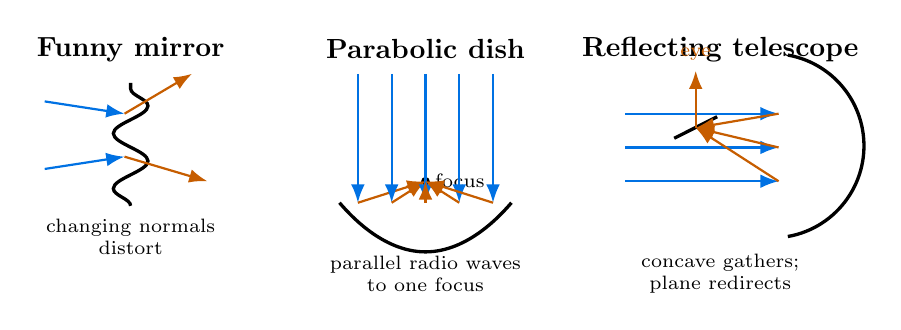
\begin{tikzpicture}[>=Latex,scale=.78,font=\scriptsize]
% funny mirror
\node[font=\bfseries] at (-4.8,2.4){Funny mirror};
\draw[very thick,decorate,decoration={snake,amplitude=2.2mm,segment length=7mm}] (-4.8,-.15)--(-4.8,1.85);
\draw[blue,-Latex,thick] (-6.2,1.55)--(-4.9,1.35); \draw[orange,-Latex,thick] (-4.9,1.35)--(-3.8,2.0);
\draw[blue,-Latex,thick] (-6.2,.45)--(-4.9,.65); \draw[orange,-Latex,thick] (-4.9,.65)--(-3.55,.25);
\node[align=center] at (-4.8,-.65){changing normals\\distort};
% dish
\node[font=\bfseries] at (0,2.4){Parabolic dish};
\draw[very thick] (-1.4,-.1) parabola bend (0,-.9) (1.4,-.1);
\fill (0,.25) circle (2pt) node[right]{focus};
\foreach \x in {-1.1,-.55,0,.55,1.1}{\draw[blue,-Latex,thick] (\x,2)--(\x,-.1);\draw[orange,-Latex,thick] (\x,-.1)--(0,.25);}
\node[align=center] at (0,-1.25){parallel radio waves\\to one focus};
% telescope
\node[font=\bfseries] at (4.8,2.4){Reflecting telescope};
\draw[very thick] (5.9,-.65) arc[start angle=-80,end angle=80,radius=1.5];
\draw[very thick] (4.05,.95)--(4.75,1.3);
\foreach \y in {.25,.8,1.35}{\draw[blue,-Latex,thick] (3.25,\y)--(5.75,\y);}
\draw[orange,-Latex,thick] (5.75,.25)--(4.4,1.12); \draw[orange,-Latex,thick] (5.75,.8)--(4.4,1.12); \draw[orange,-Latex,thick] (5.75,1.35)--(4.4,1.12);
\draw[orange,-Latex,thick] (4.4,1.12)--(4.4,2.05) node[above]{eye};
\node[align=center] at (4.8,-1.25){concave gathers;\\plane redirects};
\end{tikzpicture}
\end{center}

\begin{mistakebox}
Do not explain all three devices with the vague sentence ``the mirror reflects light.'' State what the shape achieves: changing normals distort a funny-mirror image; a parabola directs incoming waves to one focus; the telescope's curved mirror gathers and focuses a large area of light, while its plane mirror redirects the image to the eye.
\end{mistakebox}

\section*{9. Worked example: construct a periscope ray diagram}
The task was to see an object over a wall using two plane mirrors. The difficult part is planning a path that reaches the eye. Alex's recommended method was to begin at the observer's eye and work \textbf{backwards} towards the object. This is a construction strategy only; after the path is found, arrowheads must show the real direction in which light travels.

\newpage
\begin{center}
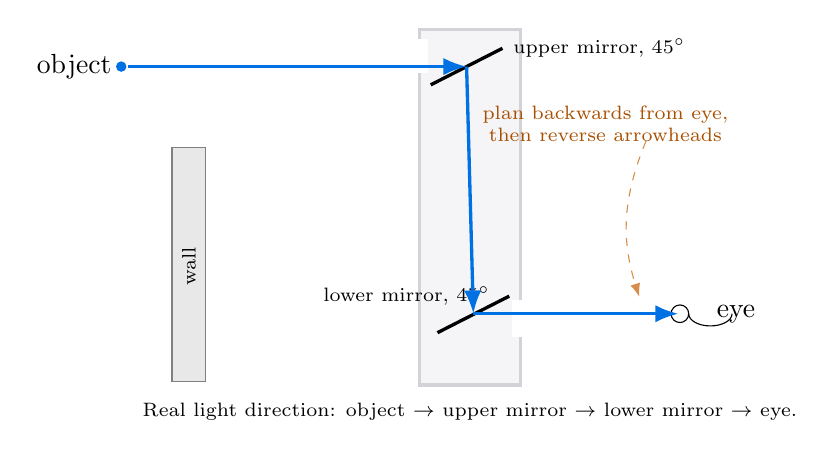
\begin{tikzpicture}[>=Latex,scale=.86]
% wall and tube
\draw[fill=gray!18,draw=gray] (-4.4,-.2) rectangle (-3.9,3.25);
\node[rotate=90,font=\scriptsize] at (-4.15,1.5){wall};
\draw[fill=soft,draw=line,very thick] (-.75,-.25) rectangle (.75,5.0);
\draw[white,line width=7pt] (-.76,4.35)--(-.76,4.85);
\draw[white,line width=7pt] (.76,.45)--(.76,1.0);
% mirrors \ orientation gives horizontal->down then down->right
\draw[very thick] (-.58,4.18)--(.48,4.72) node[right,font=\scriptsize]{upper mirror, $45^\circ$};
\draw[very thick] (-.48,.52)--(.58,1.06) node[left,xshift=-3pt,font=\scriptsize]{lower mirror, $45^\circ$};
% object and eye
\fill[blue] (-5.15,4.45) circle (2.2pt);\node[left] at (-5.15,4.45){object};
\draw (3.1,.8) circle (.13);\draw (3.23,.8) arc (180:360:.32 and .18);\node[right] at (3.5,.8){eye};
% light path real direction
\draw[blue,very thick,-Latex] (-5.05,4.45)--(-.05,4.45);
\draw[blue,very thick,-Latex] (-.05,4.45)--(.05,.8);
\draw[blue,very thick,-Latex] (.05,.8)--(3.08,.8);
% backward construction hint
\node[orange!85!black,align=center,font=\scriptsize] at (2.0,3.6){plan backwards from eye,\\then reverse arrowheads};
\draw[orange!70,dashed,-Latex] (2.6,3.35) to[bend right=20] (2.5,1.05);
\node[font=\scriptsize] at (0,-.65){Real light direction: object $\rightarrow$ upper mirror $\rightarrow$ lower mirror $\rightarrow$ eye.};
\end{tikzpicture}
\end{center}

\subsection*{Alex's eye-backwards method, step by step}
\begin{enumerate}
\item Draw the wall, the object beyond its top, the periscope tube and the observer's eye at the lower opening.
\item Place two parallel plane mirrors inside the tube, each at about $45^\circ$: one beside the upper opening and one beside the lower opening.
\item Start at the eye and sketch backwards to the centre of the lower mirror. Continue vertically up the tube to the upper mirror, then horizontally out towards the object. Working backwards makes the required destination---the eye---easy to hit.
\item Now treat that line as a real light path and reverse the planning direction. Put arrowheads from the object to the upper mirror, down the tube to the lower mirror, and finally into the eye.
\item At each mirror imagine, or draw, a local normal and check $i=r$. With the mirrors at $45^\circ$, the upper reflection turns the horizontal light down the tube; the lower reflection turns it horizontally into the eye.
\end{enumerate}

The eye does not send out the viewing ray. Starting there is only Alex's efficient way to design a route that is redirected twice.

\begin{mistakebox}
Do not leave the arrows pointing from eye to object merely because you constructed the path backwards. Real light travels from the object into the eye. Also check that both mirrors are parallel and near $45^\circ$; a path drawn through the tube without two reflections does not explain the periscope.
\end{mistakebox}

\clearpage
\section*{10. One-page quick-recall summary}
\footnotesize
\renewcommand{\arraystretch}{1.18}
\begin{tabularx}{\linewidth}{>{\bfseries}p{.22\linewidth}Y}
\toprule
Prompt & Recall answer\\
\midrule
Spectrum, low $f$ to high $f$ & Radio, microwave, infrared, visible, ultraviolet, X-ray, gamma; R--M--IR--V--UV--X--$\gamma$.\\
Frequency vs wavelength & They run in opposite directions. Radio $\rightarrow$ gamma means frequency/energy increase and wavelength decreases.\\
Why high frequency can be dangerous & From ultraviolet onwards in Alex's ordering: enough frequency/energy to remove electrons, ionising atoms; this can mutate cells and cause cancer.\\
X-ray row & Uses: see bones; industrial imaging. Danger: ionises atoms in cells; mutation--cancer.\\
Gamma row & Uses: treat cancer; sterilise equipment by killing bacteria. Danger: ionises atoms in cells; mutation--cancer.\\
Actual ordering slips & Missing IR--V--UV after microwave; nearly missing microwave before radio; starting descending wavelength at microwave rather than radio. Count all seven.\\
Visible-light extension & Eyes evolved in water where visible light was least absorbed and therefore most available; eye cells convert detected light into electrical signals for the brain.\\
Wavefront & A line joining points in the same phase: for example, every crest. Circular wavefronts are concentric; plane wavefronts are parallel.\\
Ray & Arrow showing the direction of wave/energy travel---Alex's ``surfer on the wave.'' Rays are perpendicular to wavefronts.\\
Luminous & Emits its own light: Sun, bulb, candle, fire. A visible object is not automatically luminous.\\
Transparent / opaque & Transparent transmits light, though a little may reflect. Opaque transmits none: most reflects and some is absorbed. Translucent lets some through.\\
Normal & Imaginary line at $90^\circ$ to the surface at the point of incidence. Alex's ``always'' line: always measure angles from it.\\
Law of reflection & $i=r$. Incident arrow points towards the mirror; reflected arrow points away. Both angles are from the normal.\\
Specular vs diffuse & Smooth surface: parallel normals and ordered parallel reflection. Rough surface: different local normals scatter rays. Every ray still obeys $i=r$.\\
Curved examples & Funny mirror: changing normals distort. Dish: parabola reflects incoming radio waves to one focus. Telescope: concave mirror gathers/focuses; plane mirror redirects to eye.\\
Periscope method & Plan eye $\rightarrow$ lower mirror $\rightarrow$ upper mirror $\rightarrow$ object; then draw real arrows object $\rightarrow$ upper $\rightarrow$ lower $\rightarrow$ eye. Two parallel $45^\circ$ mirrors.\\
\bottomrule
\end{tabularx}

\begin{keybox}{Final exam checklist}
\begin{itemize}
\item Translate the direction words before writing the EM order; count seven bands.
\item Explain ionising danger as a causal chain, not just ``high frequency is bad.''
\item Distinguish a wavefront (same phase) from a ray (energy direction), and make them perpendicular.
\item On every reflection diagram, draw the local normal and measure from it.
\item For diffuse reflection, preserve $i=r$ for each ray; only the local normals differ.
\item In a periscope, use eye-backwards planning but object-to-eye arrowheads.
\end{itemize}
\end{keybox}
\end{document}
